\begin{Slide}{Use cases}
\begin{itemize}
\item Definition according to \url{https://en.wikipedia.org/wiki/Use_case}
\begin{itemize}
\item  A usage scenario for a piece of software.
\item  A potential scenario in which a system receives an external request and responds to it.

\end{itemize}
\end{itemize}
\vspace{-0.5em}
\begin{minipage}[t]{0.55\textwidth}
\begin{itemize}
\item Contents of textual use case:
\begin{itemize}
\item Title
\item Primary Actor
\item Brief (corresponds to user story)
\item Stakeholders
\item Pre- and postconditions
\item Triggers
\item Basic flows
\item Extensions
\end{itemize}
\end{itemize}
\end{minipage}%
\hfill\begin{minipage}[t]{0.45\textwidth}
\vspace{-0.4em}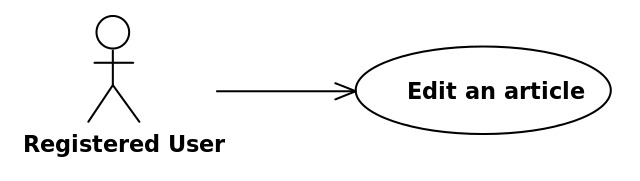
\includegraphics[width=1.0\textwidth]{../img/use-case-edit-article}
\end{minipage}
\end{Slide}
